% !TEX program = xelatex
% 공통수학2 · Ⅲ. 함수와 그래프 · 1. 함수 · 03 역함수 · 2/2차시
\documentclass[11pt,a4paper]{article}
\usepackage{kotex}
\usepackage{iftex}
\ifPDFTeX\else
  \setmainhangulfont{Noto Serif CJK KR}
  \setsanshangulfont{Noto Sans CJK KR}
\fi
\usepackage[margin=2.1cm]{geometry}
\usepackage{parskip}
\usepackage{enumitem}
\usepackage{array}
\usepackage{tabularx}
\usepackage{booktabs}
\usepackage{xcolor}
\usepackage{amssymb}
\usepackage{tikz}
\usepackage[most]{tcolorbox}
\usepackage{fancyhdr}
\usepackage{titlesec}

\definecolor{goldc}{HTML}{B07C22}
\definecolor{goldstrong}{HTML}{8A5F16}
\definecolor{indigoc}{HTML}{2B3B57}
\definecolor{indigosoft}{HTML}{6E82A6}
\definecolor{linec}{HTML}{D6DACB}
\definecolor{surface2}{HTML}{E4E8DC}
\definecolor{notebg}{HTML}{FBF3E3}
\definecolor{inksoft}{HTML}{52604F}

\titleformat{\section}{\normalfont\sffamily\bfseries\large\color{indigoc}}{\thesection}{0.6em}{}
\titlespacing{\section}{0pt}{16pt}{8pt}
\newtcolorbox{ideabox}{enhanced, breakable, colback=white, colframe=goldc, boxrule=0.5pt, leftrule=3pt, arc=2pt, left=10pt, right=10pt, top=8pt, bottom=8pt}
\newtcolorbox{calloutbox}{enhanced, breakable, colback=white, colframe=indigosoft, boxrule=0.5pt, leftrule=3pt, arc=2pt, left=10pt, right=10pt, top=7pt, bottom=7pt}
\newtcolorbox{notebox}{enhanced, breakable, colback=notebg, colframe=goldc, boxrule=0.5pt, leftrule=3pt, arc=2pt, left=10pt, right=10pt, top=7pt, bottom=7pt}
\newtcolorbox{answerbox}{enhanced, breakable, colback=white, colframe=linec, boxrule=0.5pt, arc=2pt, left=10pt, right=10pt, top=7pt, bottom=7pt}
\newcommand{\lessonbanner}[3]{%
  \begin{tcolorbox}[enhanced, colback=indigoc, colframe=indigoc, boxrule=0pt, arc=0pt,
    left=14pt, right=14pt, top=14pt, bottom=10pt, borderline south={2.4pt}{0pt}{goldc}, fontupper=\color{white}]
    {\sffamily\footnotesize\color{white!85!black} #1}\\[4pt]{\sffamily\bfseries\Large #2}\\[3pt]{\sffamily\small\color{white!88!black} #3}
  \end{tcolorbox}}
\pagestyle{fancy}\fancyhf{}\renewcommand{\headrulewidth}{0pt}
\fancyfoot[L]{\footnotesize\color{inksoft} 공통수학2 · 2026학년도 2학기 · 지평선고등학교}
\fancyfoot[R]{\footnotesize\color{inksoft} 교사용 지도안 -- 배포 금지}

\newcommand{\invgraph}{%
  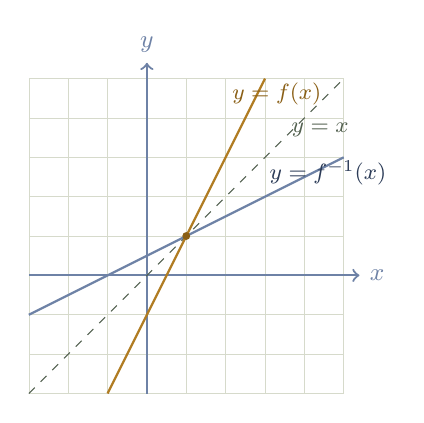
\begin{tikzpicture}[scale=0.5]
    \draw[step=1cm, linec, very thin] (-3,-3) grid (5,5);
    \draw[->, thick, indigosoft] (-3,0) -- (5.4,0) node[right, font=\small]{$x$};
    \draw[->, thick, indigosoft] (0,-3) -- (0,5.4) node[above, font=\small]{$y$};
    \draw[dashed, inksoft] (-3,-3) -- (5,5);
    \node[font=\footnotesize, inksoft] at (4.4,3.7) {$y=x$};
    \draw[thick, goldc, domain=-1:3] plot(\x,{2*\x-1});
    \node[font=\footnotesize, goldstrong] at (3.3,4.6) {$y=f(x)$};
    \draw[thick, indigosoft, domain=-3:5] plot(\x,{(\x+1)/2});
    \node[font=\footnotesize, indigoc] at (4.6,2.6) {$y=f^{-1}(x)$};
    \filldraw[goldstrong] (1,1) circle (2.4pt);
  \end{tikzpicture}}

\begin{document}
\lessonbanner{공통수학2 · Ⅲ. 함수와 그래프 · 1. 함수}{03 역함수 --- 2/2차시}{역함수의 그래프 · 교사용 지도안 (2026학년도 2학기)}
\vspace{10pt}

\noindent\begin{tabularx}{\linewidth}{@{}>{\bfseries\color{indigoc}}p{2.6cm}X@{}}
\toprule
대상 & 고1 · 2개 반 · 반당 13명 \\
차시 & 50분 (도입 10 · 전개 30 · 정리 10) \\
성취기준 & 함수와 그 역함수의 그래프 사이의 관계를 이해하고, 역함수의 그래프를 그릴 수 있다. \\
선행 학습 & 36차시 --- 역함수의 뜻과 성질, 15차시 --- 대칭이동(직선 $y=x$ 대칭) \\
\bottomrule
\end{tabularx}

\section{학습 목표 \& Big Idea}
\begin{ideabox}
\textbf{\color{goldstrong}영속적 이해 (Big Idea)}\\
함수와 그 역함수는 $x$와 $y$의 역할을 서로 맞바꾼 관계이므로, 두 그래프는 언제나 직선 $y=x$에 대하여 대칭이다. 대칭이동이라는 옛 개념이 역함수라는 새 개념 속에서 다시 살아난다.
\vspace{4pt}
\small\color{inksoft} 핵심개념: \textbf{대칭성} \quad\textbullet\quad 핵심개념: \textbf{좌표의 교환} \quad\textbullet\quad 일반화: \textbf{역함수는 원래 함수를 $y=x$에 대하여 비춘 거울상이다}
\end{ideabox}
\begin{calloutbox}
\textbf{차시 학습 목표}
\begin{itemize}[leftmargin=1.4em, itemsep=2pt, topsep=4pt]
  \item 함수 $f$의 그래프 위의 점 $(a,b)$가 역함수 $f^{-1}$의 그래프 위의 점 $(b,a)$에 대응함을 알고, 두 그래프가 직선 $y=x$에 대하여 대칭임을 설명할 수 있다.
  \item 함수의 그래프로부터 그 역함수의 그래프를 그리고, 두 그래프의 교점을 구할 수 있다.
\end{itemize}
\end{calloutbox}

\section{질문의 연결}
\begin{tabularx}{\linewidth}{@{}>{\bfseries\color{indigoc}\small}p{2.4cm}X@{}}
사실적 질문 & $y=f(x)$의 그래프가 주어졌을 때 $y=f^{-1}(x)$의 그래프는 어떻게 그릴 수 있을까? \\[6pt]
개념적 질문 & 왜 함수와 그 역함수의 그래프는 항상 직선 $y=x$에 대하여 대칭일까? \\[6pt]
논쟁적 질문 & 거울에 비친 나의 모습은 `나의 역함수'라고 부를 수 있을까? 수학의 역함수와 거울 대칭은 어디까지 같고 어디서 달라질까? \\
\end{tabularx}

\section{수업 흐름}
\begin{tabularx}{\linewidth}{@{}>{\centering\arraybackslash}p{1.6cm}X>{\raggedright\arraybackslash\small}p{3.1cm}@{}}
\toprule
\textbf{단계} & \textbf{활동 \& 발문} & \textbf{ATL / VTR} \\
\midrule
\textcolor{goldstrong}{\textbf{도입}}\newline\footnotesize 10분 &
\textbf{마음공부 (2분)} --- 유무념 대조.\newline
\textbf{생각 열기 (8분)} --- 15차시에서 배운 `점 $(a,b)$를 직선 $y=x$에 대하여 대칭이동하면 $(b,a)$'를 복습하고, 이것이 오늘 배울 역함수와 어떤 관계가 있을지 예측. &
ATL: 사고(선행 개념 연결)\newline VTR: See-Think-Wonder \\
\addlinespace
\textcolor{goldstrong}{\textbf{전개}}\newline\footnotesize 30분 &
\textbf{대칭성의 원리 (10분)} --- $(a,b)$가 $y=f(x)$ 위의 점 $\iff$ $f(a)=b$ $\iff$ $f^{-1}(b)=a$ $\iff$ $(b,a)$가 $y=f^{-1}(x)$ 위의 점, 이라는 논리 사슬로 두 그래프가 $y=x$ 대칭임을 유도.\newline
\textbf{역함수 그래프 그리기 (12분)} --- $f(x)=2x-1$의 그래프를 그리고, 이를 $y=x$에 대하여 대칭이동해 $f^{-1}(x)=\frac{x+1}{2}$의 그래프를 완성 $\to$ 문제 1.\newline
\textbf{교점 구하기 (8분)} --- 증가함수일 때 교점은 항상 $y=x$ 위에 있으므로 $f(x)=x$를 풀면 됨을 확인 $\to$ 문제 2, 문제 3. &
ATT: 촉진자 역할\newline ATL: 기하적 추론·대수적 확인 \\
\addlinespace
\textcolor{goldstrong}{\textbf{정리}}\newline\footnotesize 10분 &
\textbf{개념 연결 질문 (5분)} --- ``함수와 그 역함수의 그래프의 교점이 항상 $y=x$ 위에 있다고 할 수 있을까?''\newline
\textbf{성찰 (5분)} --- 감사 일기 1문장 + 다음 차시 예고(중단원 마무리: 함수 전체 종합). &
마음공부 · 감사 일기 \\
\bottomrule
\end{tabularx}

\begin{calloutbox}
\textbf{지도상의 유의점} --- 교점을 구할 때 무조건 $f(x)=x$를 풀면 된다고 오해하기 쉽다. 이는 $f$가 \textbf{증가함수}일 때만 보장되는 사실이며, 감소함수인 경우에는 교점이 $y=x$ 위에 있지 않을 수도 있음을 문제 4에서 개념적으로 짚어 준다.
\end{calloutbox}

\section{형성평가 \& 답안}
\begin{answerbox}
\textbf{문제 1} \quad $f(x)=2x-1$의 역함수를 구하고, 두 함수의 그래프를 한 좌표평면 위에 그리시오.

\vspace{4pt}
\centering \invgraph

\vspace{4pt}
\raggedright\textbf{\color{goldstrong}답} \; $f^{-1}(x)=\dfrac{x+1}{2}$. 두 그래프는 직선 $y=x$(점선)에 대하여 대칭이며, 교점은 $(1,1)$.
\end{answerbox}

\vspace{6pt}
\begin{minipage}[t]{0.48\linewidth}
\begin{answerbox}
\textbf{문제 2} \quad 증가함수 $f(x)=x^3$의 그래프와 그 역함수의 그래프의 교점을 모두 구하시오.\\[4pt]
\textbf{\color{goldstrong}답} \; 증가함수이므로 $f(x)=x$를 풀면 됨. $x^3=x \Rightarrow x(x-1)(x+1)=0 \Rightarrow x=-1,0,1$. 교점: $(-1,-1)$, $(0,0)$, $(1,1)$.
\end{answerbox}
\end{minipage}\hfill
\begin{minipage}[t]{0.48\linewidth}
\begin{answerbox}
\textbf{문제 3} \quad $f(x)=\frac12x+2$의 그래프와 역함수의 그래프가 만나는 점을 구하시오.\\[4pt]
\textbf{\color{goldstrong}답} \; 증가함수이므로 $\frac12x+2=x \Rightarrow x=4$. 교점: $(4,4)$.
\end{answerbox}
\end{minipage}

\vspace{6pt}
\begin{answerbox}
\textbf{문제 4 (개념 서술형)} \quad ``함수와 그 역함수의 그래프의 교점은 항상 직선 $y=x$ 위에 있다.''라는 문장의 참·거짓을 판단하고 근거를 서술하시오.\\[4pt]
\textbf{\color{goldstrong}답} \; 거짓(일반적으로는 아님). $f$가 \textbf{증가함수}이면 교점이 항상 $y=x$ 위에 있음이 보장되지만, $f$가 \textbf{감소함수}인 경우에는 반드시 그렇지 않다 --- 감소함수 중에는 $y=x$ 위에 있지 않은 점에서 그래프가 만나는 경우도 있다.
\end{answerbox}

\section{성취수준 (이 차시 범위)}
\begin{tabularx}{\linewidth}{@{}>{\bfseries\color{goldstrong}}p{0.9cm}X@{}}
\toprule
A & 그래프 대칭의 원리를 논리적으로 설명하고, 증가함수·감소함수에 따른 교점의 성질 차이를 근거를 들어 설명할 수 있다. \\
B & 함수의 그래프로부터 역함수의 그래프를 정확히 그리고, 두 그래프의 교점을 구할 수 있다. \\
C & 직선 $y=x$에 대한 대칭임을 알고, 안내에 따라 역함수의 그래프를 그릴 수 있다. \\
D & 주어진 두 그래프가 $y=x$ 대칭임을 확인할 수 있다. \\
E & 역함수의 그래프가 원래 함수의 그래프와 관련 있음을 안다. \\
\bottomrule
\end{tabularx}

\section{다음 차시}
\begin{calloutbox}
\textbf{중단원 마무리 (함수) --- 38차시.} 33$\sim$37차시(함수의 뜻, 여러 가지 함수, 합성함수, 역함수)를 종합 정리하고 형성평가로 점검한다.
\end{calloutbox}
\end{document}
